
%(BEGIN_QUESTION)
% Copyright 2014, Tony R. Kuphaldt, released under the Creative Commons Attribution License (v 1.0)
% This means you may do almost anything with this work of mine, so long as you give me proper credit

Bruk Kirchhoffs strømlov til å beregne størrelser og retninger for strømmer gjennom {\it alle} motstandene i denne kretsen:

$$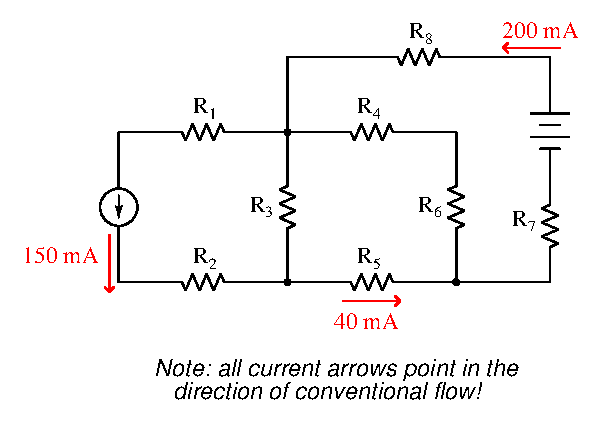
\includegraphics[width=15.5cm]{i01162x01.eps}$$

\vfil 

\underbar{file i01162}
\eject
%(END_QUESTION)





%(BEGIN_ANSWER)

Dette er en vurderingsoppgave -- ingen svar eller hint er gitt!

%(END_ANSWER)





%(BEGIN_NOTES)

Det er ikke nødvendig å kunne serie-parallellkretser, eller engang parallellkretser, for å finne strømmen gjennom $R_4$ -- det holder å kunne bruke Kirchhoffs strømlov:

$$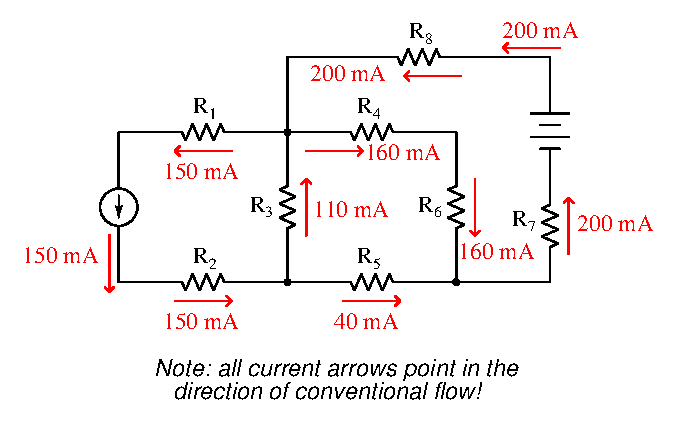
\includegraphics[width=15.5cm]{i01162x02.eps}$$

%INDEX% Elektronikkrepetisjon: serie-parallellkretser

%(END_NOTES)

